\documentclass[aps,prb,twocolumn,superscriptaddress,floatfix,longbibliography,10pt]{revtex4-2}

\usepackage[utf8]{inputenc}
\usepackage[spanish]{babel}
\usepackage{graphicx}
\usepackage{amsmath}
\usepackage{subcaption}
\usepackage{wrapfig} 
\usepackage[export]{adjustbox}

\usepackage{amsmath,amssymb} % math symbols
\usepackage{bm} % bold math font
\usepackage{graphicx} % for figures
\usepackage{comment} % allows block comments
\usepackage{textcomp} % This package is just to give the text quote '
%\usepackage{ulem} % allows strikeout text, e.g. \sout{text}

\usepackage[spanish]{babel}
% By dafault, spanish changes to a comma as decimal separator; to change to a dot, you can use \decimalpoint:
\decimalpoint

\usepackage{enumitem}
\setlist{noitemsep,leftmargin=*,topsep=0pt,parsep=0pt}

\usepackage{xcolor} % \textcolor{red}{text} will be red for notes
\definecolor{lightgray}{gray}{0.6}
\definecolor{medgray}{gray}{0.4}

%Para las tablas
\usepackage{multirow}

\usepackage{hyperref}
\hypersetup{
colorlinks=true,
urlcolor= blue,
citecolor=blue,
linkcolor= blue,
bookmarks=true,
bookmarksopen=false,
}

% Code to add paragraph numbers and titles
\newif\ifptitle
\newif\ifpnumber
\newcounter{para}
\newcommand\ptitle[1]{\par\refstepcounter{para}
{\ifpnumber{\noindent\textcolor{lightgray}{\textbf{\thepara}}\indent}\fi}
{\ifptitle{\textbf{[{#1}]}}\fi}}
% \ptitletrue  % comment this line to hide paragraph titles
% \pnumbertrue  % comment this line to hide paragraph numbers

% minimum font size for figures
\newcommand{\minfont}{6}

% Uncomment this line if you prefer your vectors to appear as bold letters.
% By default they will appear with arrows over them.
% \renewcommand{\vec}[1]{\bm{#1}}

%Cambiar Cuadros por Tablas y lista de...
%\renewcommand{\listtablename}{Índice de tablas}
\renewcommand{\tablename}{Tabla}
\renewcommand{\date}{Fecha}

%Para importar imágenes desde una carpeta:
\graphicspath{ {C:/Users/lupam/OneDrive/Escritorio/GitHub/Metodos_Num_Fluidos_I/Guias/Guia_2/Ejercicio_4/Programa/graficos} {C:/Users/lupam/OneDrive/Escritorio/GitHub/Metodos_Num_Fluidos_I/Guias/Guia_2/Ejercicio_4/Informe/Figures}}


\usepackage[bottom]{footmisc} %para que las notas al pie aparezcan en la misma página

\begin{comment}

%Comandos de interés:

* Para ordenar el documento:
\section{Introducción}
\section{\label{sec:Formatting}Formatting} %label para luego hacer referencia a esa sección

\ptitle{Start writing while you experiment} %pone nombre y título al documento dependiendo de si en el header están los comandos \ptitletrue y \pnumbertrue

* Ecuaciones:
\begin{equation}
a^2+b^2=c^2 \,.
\label{eqn:Pythagoras}
\end{equation}

* Conjunto de ecuaciones:
\begin{eqnarray}
\label{eqn:diagonal}
\nonumber d & = & \sqrt{a^2 + b^2 + c^2} \\
& = & \sqrt{3^2+4^2+12^2} = 13
\end{eqnarray}

* Para hacer items / enumerar:
\begin{enumerate}
  \item
\end{enumerate}

\begin{itemize}
  \item
\end{itemize}

* Figuras:
\begin{figure}[h]
    \includegraphics[clip=true,width=\columnwidth]{pixel-compare}
    \caption{}
     \label{fig:pixels}
\end{figure}

* Conjunto de figuras:
(no recuerdo)


* Para hacer referencias a fórmulas, tablas, secciones, ... dentro del documento:
\ref{tab:spacing}

* Para citar
Elementos de .bib
\cite{WhitesidesAdvMat2004}
url
\url{http://www.mendeley.com/}\\

* Agradecimientos:
\begin{acknowledgments}
We acknowledge advice from Jessie Zhang and Harry Pirie to produce Fig.\ \ref{fig:pixels}.
\end{acknowledgments}

* Apéndice:
\appendix
\section{\label{app:Mendeley}Mendeley}

* Bibliografía:
\bibliography{Hoffman-example-paper}

\end{comment}



\begin{document}

% Allows to rewrite the same title in the supplement
\newcommand{\mytitle}{Laboratorio 2 - Problema de valores iniciales}

\title{\mytitle}

\author{Pablo Chehade \\
    \small \textit{pablo.chehade@ib.edu.ar} \\
    \small \textit{Métodos Numéricos en Fluidos I, Instituto Balseiro, CNEA-UNCuyo, Bariloche, Argentina, 2022} \\}


\begin{abstract}

Se estudiaron distintos métodos numéricos para resolver problemas de valores iniciales no lineales. En particular se aplicaron los métodos de Euler implícito, Crank-Nicholson, Runge-Kutta 4 y una combinación de Crank-Nisholson con Leap-Frog al problema del péndulo simple y el método de Runge-Kutta 4 al del péndulo doble. En el caso del péndulo simple se analizaron los errores fase y amplitud globales de cada método, se calcularon los órdenes de convergencia y se compararon con los valores teóricos. En el caso del péndulo doble se analizó la sensibilidad del sistema frente a perturbaciones y el error de amplitud global.
\end{abstract}

\maketitle

\section{Introducción}

\ptitle{¿Por qué es importante estudiar numéricamente PVI?}
\ptitle{En este trabajo se analizaron dos problemas de valores iniciales}

En ciencias físicas es de gran interés conocer la dinámica de un sistema a partir de sus condiciones iniciales. Sin embargo, dadas las ecuaciones de movimiento, no siempre es posible obtener la dinámica exactamente y es necesario recurrir a métodos numéricos. Existen una gran variedad de esquemas numéricos y ninguno está excento de error. En este trabajo se analizaron dos problemas de valores iniciales: la evolución del péndulo simple y del péndulo doble. Se resolvieron numéricamente a través de distintos métodos numéricos implícitos y explícitos y se estudió la convergencia de los mismos.

\subsection{Péndulo simple}

\ptitle{Presentar ecuaciones de la dinámica}

\begin{figure}[h]
  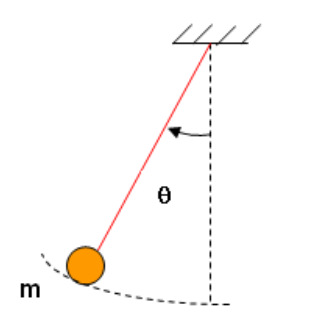
\includegraphics[clip=true,width=0.6\columnwidth]{simple_esquema.png}
  \caption{Esquema del péndulo simple. Una partícula puntual de masa $m$ está suspendida de un punto fijo mediante un hilo de longitud $l$. El ángulo $\theta$ es el ángulo que forma el hilo con la vertical. Imagen extraída de \cite{esquema_pendulo_simple}.}
   \label{fig:simple_esquema}
\end{figure}
% 

El péndulo simple consta de una partícula puntual de masa $m$ suspendida de un punto fijo mediante un hilo de longitud $l$ (ver esquema en figura \ref{fig:simple_esquema}). La partícula se mueve en un plano y el ángulo $\theta$ que forma el hilo con la vertical se describe mediante la ecuación diferencial
\begin{equation}
  \left\{\begin{matrix}
    \theta'' = -\frac{g}{l} \sin{(\theta)} \\
    \theta(0) = \theta_0, \theta'(0) = \theta'_0
   \end{matrix}\right.
  \label{eq:pendulo_simple}
\end{equation}
donde $g$ es la aceleración de la gravedad y $\theta_0$ y $\theta'_0$ corresponden a las condiciones iniciales de ángulo y velocidad angular, respectivamente. Algunos parámetros importantes de la evolución de este sistema en particular son el período de oscilación $\tau$ dado por \cite{periodo_exacto_pendulo_simple}
\begin{equation}
  \tau(\theta) = T_0 \left [ \sum_{n = 0}^\infty \left(  \frac{(2n)!}{2^{2n}(n!)^2} \right )^2 \sin^{2n} \left ( \frac{\theta}{2} \right )   \right ], T_0 = 2 \pi \sqrt{\frac{l}{g}},
  \label{eq:periodo_simple}
\end{equation}
la fase $\phi_{teo}$ dada por
\begin{equation}
  \phi_{teo}(\theta) = \tan^{-1}(\theta'/\theta)
  \label{eq:fase_simple}
\end{equation}
y la energía por unidad de masa o amplitud $A_S$ dada por
\begin{equation}
  A^S(\theta) = 1/2 l^2 \theta'^2 - g l \cos{(\theta)}.
  \label{eq:amplitud_simple}
\end{equation}
Debido a que solo actúan fuerzas conservativas, la amplitud $A_S$ se mantiene constante durante la evolución.

\ptitle{Ecuación vectorial del péndulo simple}

La ecuación diferencial de segundo orden de \ref{eq:pendulo_simple} se puede convertir en dos ecuaciones diferenciales de orden 1 mediante el cambio de variable $\vec{y}_S^T = (y_1, y_2) =  (\theta, \theta')$. De este modo, el problema \ref{eq:pendulo_simple} se convierte en

\begin{equation}
  \left\{\begin{matrix}
    \frac{d\vec{y_S}}{dt}  = 
    \begin{pmatrix}
    y_2 \\ -\frac{g}{l} \sin{y_1}
    \end{pmatrix}
    = \vec{f_S}(\vec{y_S},t), 
  \\
  \vec{y}_S(0) = 
  \begin{pmatrix}
    \theta_0 \\ \theta'_0
      \end{pmatrix}
  \end{matrix}\right.
  \label{eq:pendulo_simple_vec}
\end{equation}

% \begin{equation}
%   \left\{\begin{matrix}
%     \frac{d\vec{y_S}}{dt}  = 
%     \begin{pmatrix}
%     y_2 \\ -\frac{g}{l} \sin{y_1}
%     \end{pmatrix}
%     = \vec{f_S}(\vec{y_S},t), 
%   \\
%     \vec{y}_S^T(0) = (\theta_0, \theta'_0).
%   \end{matrix}\right.
%   \label{eq:pendulo_simple_vec}
% \end{equation}

\subsection{Péndulo doble}

\ptitle{Presentar ecuaciones de la dinámica}

\begin{figure}[h]
  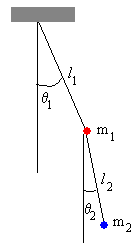
\includegraphics[clip=true,width=0.6\columnwidth]{doble_esquema.png}
  \caption{Esquema del péndulo doble. Una partícula puntual de masa $m_1$ está suspendida de un punto fijo mediante un hilo de longitud $l_1$. El ángulo $\theta_1$ es el ángulo que forma el hilo con la vertical. Sobre esta partícula se encuentra suspendida otra de masa $m_2$ mediante un hilo de longitud $l_2$. El ángulo $\theta_2$ es el ángulo que forma este último hilo con la vertical. Imagen extraída de \cite{Notas_materia}.}
   \label{fig:doble_esquema}
\end{figure}



El péndulo doble es un sistema más complejo que el anterior. Consta básicamente de un péndulo simple con masa $m_1$, longitud $l_1$ y ángulo $\theta_1$ sobre el que se suspende otro péndulo con masa $m_2$, longitud $l_2$ y ángulo $\theta_2$ (ver esquema en la figura \ref{fig:doble_esquema}). Empleando $l_1 = l_2 = 1$, $m_1 = m_2 = 1$ y $g = 10$, las ecuaciones de la evolución de los ángulos involucrados son
\begin{equation}
\left\{\begin{matrix}
  2 \theta_1'' + \theta_2'' \cos{\Delta \theta} = \theta_2'^2 \sin{\Delta \theta} - 20 \sin{(\theta_1)}, \\
  \theta_1'' \cos{\Delta \theta} + \theta_2'' = - \theta_1'^2 \sin{\Delta \theta} - 10 \sin{(\theta_2)}, \\
  \theta_1(0) = \theta_{1 0}, \theta_1'(0) = \theta_{1 0}', \\
  \theta_2(0) = \theta_{2 0}, \theta_2'(0) = \theta_{2 0}',
  \end{matrix}\right.
  \label{eq:pendulo_doble}
\end{equation}
donde $\Delta \theta = (\theta_2 - \theta_1)$.

Al igual que en el péndulo simple, la energía se conserva y la amplitud $A_D$ se mantiene constante durante la evolución. En este caso, tal amplitud está dada por
\begin{equation}
  A_D = \theta_1'^2 + \frac{1}{2} \theta_2'^2 + \theta_1' \theta_2' \cos{(\theta_2 - \theta_1)} - 20 \cos{\theta_1} - 10 \cos{\theta_2}
  \label{eq:amplitud_doble}
\end{equation}

\ptitle{Ecuación vectorial del péndulo doble}
Haciendo el cambio de variables $\vec{y}_D^T = (y_1, y_2, y_3, y_4) = (\theta_1, \theta_2, \theta_1', \theta_2')$, el problema \ref{eq:pendulo_doble} se convierte en

\begin{eqnarray}
  \left\{\begin{matrix}
     \frac{d\vec{y_D}}{dt} & = &
      \begin{pmatrix}
        y_3 \\
        y_4 \\
        \frac{y_4^2 \sin{\Delta} - 20 \sin{y_1} + y_3^2 \sin{\Delta} \cos{\Delta} + 10 \sin{y_2} \cos{\Delta}}{  2 - \cos^2{\Delta}  } \\
        \frac{-2 y_3^2 \sin{\Delta} - 20 \sin{y_2} - y_4^2 \sin{\Delta} \cos{\Delta} + 20 \sin{y_1} \cos{\Delta}}{  2 - \cos^2{\Delta}  }
      \end{pmatrix} \\
     & = & \vec{f_D}(\vec{y_D},t),
    \\ \\
    \vec{y}_S^T(0) & = &
    (\theta_{1 0}, \theta_{2 0}, \theta'_{1 0}, \theta'_{2 0})
  \end{matrix}\right.
  \label{eq:pendulo_doble_vec}
\end{eqnarray}
  % -y_3^2 \sin{\Delta} -10 \sin{y_2} - f_3 \cos{\Delta}

% \begin{eqnarray}
%   \label{eq:pendulo_doble_vec}
%   \left\{\begin{matrix}
%     \nonumber \frac{d\vec{y_D}}{dt} & = &
%     \begin{pmatrix}
%       y_3 \\
%       y_4 \\
%       \frac{y_4^2 \sin{\Delta} - 20 \sin{y_1} + y_3^2 \sin{\Delta} \cos{\Delta} + 10 \sin{y_2} \cos{\Delta}}{  2 - \cos^2{\Delta}  } \\
%       \frac{-2 y_3^2 \sin{\Delta} - 20 \sin{y_2} - y_4^2 \sin{\Delta} \cos{\Delta} + 20 \sin{y_1} \cos{\Delta}}{  2 - \cos^2{\Delta}  }
%     \end{pmatrix}
%     = \vec{f_D}(\vec{y_D},t), \\
%     \vec{y}_S(0) =
%     \begin{pmatrix}
%       \theta_{1 0} \\ \theta_{2 0}  \\ \theta'_{1 0} \\ \theta'_{2 0}
%      \end{pmatrix},
%     \end{matrix}\right.
%    \end{matrix}\right.
% \end{eqnarray}
%   % -y_3^2 \sin{\Delta} -10 \sin{y_2} - f_3 \cos{\Delta}
% donde $\vec{y}_D^T = (y_1, y_2, y_3, y_4)$


\section{Método Numérico}

\ptitle{Para resolver estos problemas se usaron métodos numéricos. De cada método se analizó el error de fase y el error de amplitud}

Para resolver numéricamente ambos problemas de valores iniciales es necesario discretizar la variable temporal y proponer un esquema numérico que permita obtener la solución aproximada. En cuanto a lo primero, el dominio se discretizó con puntos equiespaciados $t_n = n h$ donde $n = 0, \dots , N$ y $h = 1/N$. En cuanto a lo segundo, se utilizaron en total cuatro métodos numéricos, algunos explícitos y otros implícitos, que serán descriptos próximamente.

Además, es necesario evaluar de alguna manera la convergencia de los métodos numéricos. Para esto se podría emplear el error respecto a la solución exacta a todo tiempo o bien evaluar el error en un tiempo específico sobre cantidades conocidas. En este trabajo se optó por la segunda opción. Se evaluó para el péndulo simple el error de fase en $t = \tau$ dado por
\begin{equation}
  e^S_{fase}(t = \tau) = \phi_{aprox}(\tau) - \phi_{teo}(\tau) = \phi_{aprox}(\tau)
  \label{eq:simple_e_fase}
\end{equation}
pues por definición $\theta'(\tau) = 0$, y el error de amplificación en $t = \tau$ dado por
\begin{equation}
  e^S_{amp}(t = \tau) = A^S_{aprox}(\tau) - A^S_{teo}(\tau),
  \label{eq:simple_e_amp}
\end{equation}
donde $A^S_{teo}$ es constante como se mencionó en la sección anterior. En ambos casos, para determinar $\tau$ se empleó la expresión \ref{eq:periodo_simple} calculada con un error del orden de $10^{-15}$ menor a todos los errores obtenidos en este trabajo. Mientras que para el péndulo doble se evaluó sólo el error de amplitud para todo tiempo
\begin{equation}
  e^D_{amp}(t) = A^D_{aprox}(t) - A^D_{teo}(t),
  \label{eq:doble_e_amp}
\end{equation}
donde $A^D_{teo}$ también es constante en el tiempo.

Tanto el error de fase como el de amplitud dependen del método numérico a utilizar. Se encuentran tabulados sus órdenes de convergencia teóricos en \cite{Notas_materia}, los cuales se obtienen al analizar la ecuación diferencial $y' = \lambda y$ con $\lambda$ constante.

En base a lo anterior, a continuación se desarrollan los métodos numéricos utilizados, junto con los órdenes de convergencia globales del error de amplificación o error de amplitud y del error de fase. Es necesario aclarar que en el caso de los métodos implícitos se utilizó el método de bisección para resolver el sistema de ecuaciones resultantes, con un error del orden de $10^{-15}$ menor a todos los errores obtenidos en este trabajo.
\begin{itemize}
  \item Euler implícito (EI): este método es implícito, el factor de amplificación converge con orden $O(h^1)$ y el error de fase, con orden $O(h^2)$. Su fórmula es
  \begin{equation}
    \nonumber \vec{y}_{n+1} = \vec{y}_n + h \vec{f}(\vec{y}_{n+1}, t_{n+1}) + O_{local}(h^2)
    \label{eq:Euler_implicito}
  \end{equation}

  \item Crank-Nicholson (CN): este método es implícito, el factor de amplificación es 1, por lo que se esperaría $e^S_{amp} = 0$ y el error de fase converge con orden $O(h^2)$. Su fórmula es
  \begin{equation}
    \nonumber \vec{y}_{n+1} = \vec{y}_n + \frac{h}{2} [ \vec{f}(\vec{y}_{n+1}, t_{n+1}) + \vec{f}(\vec{y}_{n}, t_{n}) ]+ O_{local}(h^3)
    \label{eq:Crank_Nicholson}
  \end{equation}

  \item Runge Kutta 4 (RK4): este método es explícito, el factor de amplificación converge con orden $O(h^5)$ y el error de fase, con orden $O(h^4)$. Su fórmula es
  \begin{equation}
    \nonumber \vec{y}_{n+1} = \vec{y}_n + \frac{1}{6} \vec{k}_1 + \frac{1}{3} (\vec{k}_2 + \vec{k}_3) + \frac{1}{6} \vec{k}_4 + O_{local}(h^5)
    \label{eq:Runge_Kutta_4}
  \end{equation}
  donde
  \[
    \left\{\begin{matrix}
      \vec{k}_1 = h \vec{f}(\vec{y}_n, t_n), \\ 
      \vec{k}_2 = h \vec{f} \left( \vec{y}_n + \frac{1}{2} \vec{k}_1 , t_n + \frac{h}{2}\right), \\
      \vec{k}_3 = h \vec{f} \left ( \vec{y}_n + \frac{1}{2} \vec{k}_2 , t_n + \frac{h}{2}  \right ), \\
      \vec{k}_4 = h \vec{f}(\vec{y}_n + \vec{k}_3, t_n + h)
    \end{matrix}\right.
  \]

  \item 2 pasos con Crank-Nicholson y uno con Leap Frog (CN + LF). Este último método es explícito, el factor de amplificación es unitario y el error de fase converge con orden $O(h^2)$. Su fórmula es
  \begin{equation}
    \nonumber \vec{y}_{n+1} = \vec{y}_{n-1} + 2 h \vec{f}(\vec{y}_n, t_n) + O_{local}(h^3)
    \label{eq:Leap_Frog}
  \end{equation}
  El objetivo de combinar ambos métodos de esta forma en particular es que los errores de fase se compensan para dar un orden de convergencia mayor, de al menos $O(h^3)$. Además, el factor de amplificación se mantendría unitario.


\end{itemize}

\ptitle{Resumen de lo que se hará. Qué se resuelve con qué}
Se resolvió el péndulo simple con los cuatro esquemas numéricos mencionados. Se evaluó el orden de convergencia de $e^S_{fase}$ y $e^S_{amp}$ y se comparó con los valores teóricos. Además, se resolvió el péndulo doble con el método Runge-Kutta 4. Se estudió la sensibilidad del sistema frente a perturbaciones y la conservación de la amplitud.





\section{Resultados y discusión}

\subsection{Péndulo simple}

Se resolvió el péndulo simple con los cuatro esquemas numéricos mencionados para las condiciones iniciales $\theta_0 = \pi/2$ y $\theta'_0 = 0$ con $h = 0.1$. La evolución de $\theta(t)$ se grafica en la figura \ref{fig:sol_aprox}. Por un lado, se observa que la amplitud de variación de $\theta(t)$, relacionada con la amplitud $A^S$, no es constante para algunos métodos, siendo el caso más notable el de Euler implícito. Por otro lado, para algunos métodos se observa un cambio en la fase, es decir, el tiempo en el que $\theta(t)$ alcanza su valor máximo. Ambos resultados son esperados considerando el análisis de errores realizado en la sección anterior.


\begin{figure}[h]
  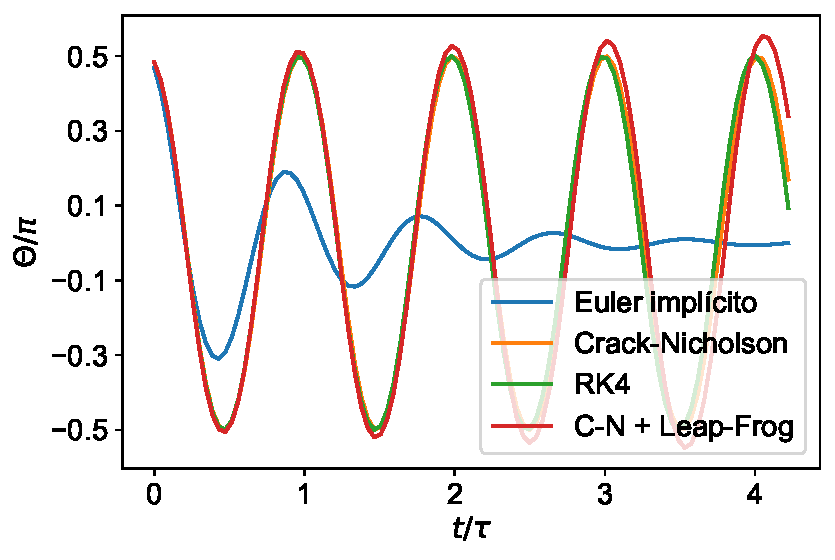
\includegraphics[clip=true,width=\columnwidth]{sol_aprox.pdf}
  \caption{Evolución de $\theta(t)$ para los cuatro esquemas numéricos para las condiciones iniciales $\theta_0 = \pi/2$ y $\theta'_0 = 0$ con $h = 0.1$. Ambos ejes se encuentran normalizados: el eje vertical por $\pi$ y el horizontal por el período $\tau$.}
   \label{fig:sol_aprox}
\end{figure}

Para todos los métodos se calculó $e^S_{fase}$ para distintos valores de $h$ y se determinó el orden de convergencia. La dependencia del error con el tamaño de la discretización para todos los esquemas se grafica en la figura \ref{fig:error_fase_simple_pi2} en escala log-log. En todos los casos se obtuvo un comportamiento lineal a partir de $h$ suficientemente pequeño. En base a esto, se ajustó una recta para cada caso, obteniendo el orden de convergencia como la pendiente de la recta. Estos se resumen en la tabla \ref{tabla:simple_errores}. Se observa que en todos los métodos los órdenes de convergencia teóricos y numéricos son distinguibles a más de 3 desviaciones estándar, siendo los más cercanos los de CN y RK4.


Análogamente, se calculó $e^S_{amp}$ en función de $h$ y se determinó el orden de convergencia. Tal dependencia se grafica en la figura \ref{fig:error_amplitud_simple_pi2}. A diferencia del caso anterior, si bien se observa un comportamiento lineal, para $h$ suficientemente pequeño, los métodos RK4 y CN alcanzan un valor constante, lo cual puede deberse a errores de punto flotante. De todos modos, se realiza un ajuste lineal sobre la zona con compotamiento lineal y se determina el orden de convergencia. Los valores se resumen en la tabla \ref{tabla:simple_errores}. Al igual que en $e^S_{fase}$, los órdenes de convergencia teóricos y numéricos son distinguibles a más de 3 desviaciones estándar. Los casos más extremos corresponden a CN y CN + LF en los que se hubiera esperado un error de amplitud nulo. Aún así, el orden de convergencia de CN es relativamente alto respecto a los demás.


En el análisis de ambos errores no se obtuvieron los órdenes de convergencia teóricos. Esto pudo deberse a que los valores teóricos se calculan en base a un problema lineal $y' = \lambda y$. En el caso de la ecuación de movimiento, el problema es no lineal y por lo tanto se puede esperar que los órdenes de convergencia no sean los mismos. Sin embargo, sí se esperaría obtener los mismos valores para $\theta_0 \rightarrow 0$ debido a que en este caso la ecuación de movimiento se reduce a un problema lineal. En base a esto se calculó la dependencia de $e^S_{fase}$ y $e^S_{amp}$ en función de $h$ para $\theta_0 = 0.01$. Los resultados se grafican en las figuras \ref{fig:error_fase_simple_angulo_bajo} y \ref{fig:error_amplitud_simple_angulo_bajo}, respectivamente. Cualitativamente se encuentran tendencias similares respecto al caso $\theta_0 = \pi/2$. La diferencia más notable se encuentra en $e^S_{amp}$ para el método de CN. Existe un valor de $h$ a partir del cual $e^S_{amp} = 0$. Esto implica que el método conserva la amplitudm bajo esas condiciones, como se esperaría a partir del análisis teórico. Es necesario aclarar que existe un valor de $h$ aún más pequeño con el cual $e^S_{amp} \neq 0$, el cual podría deberse a errores de punto flotante.


% \begin{figure}[h]
%   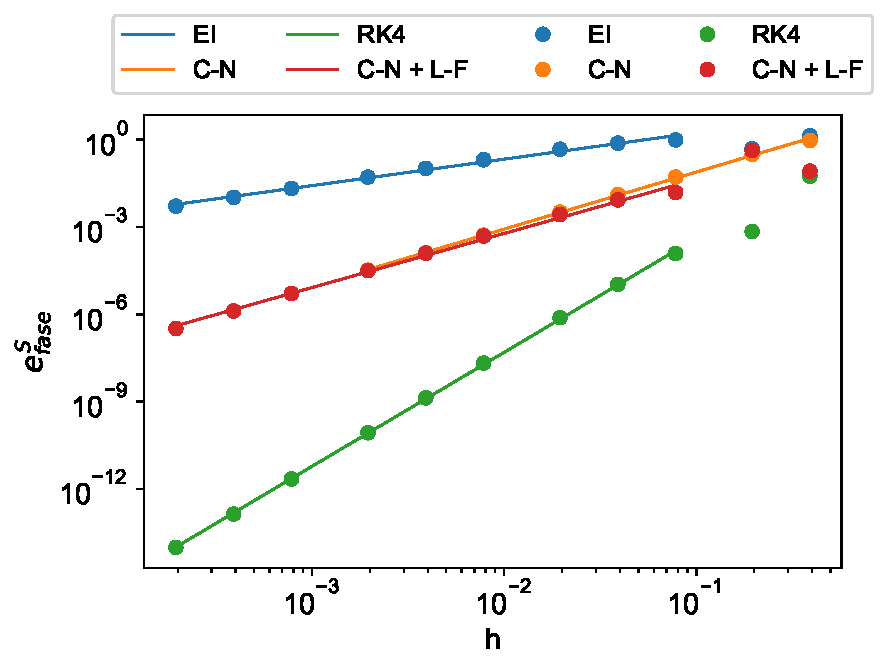
\includegraphics[clip=true,width=\columnwidth]{error_fase_simple_pi2.pdf}
%   \caption{Error de fase $e^S_{fase}$ para los cuatro esquemas numéricos en función del tamaño de la discretización $h$ bajo las condiciones iniciales $\theta_0 = \pi/2$ y $\theta'_0 = 0$. Los puntos corresponden a los valores calculados y las líneas a los ajustes lineales. 'EI': Euler implícito, 'C-N': Crank-Nicholson, 'RK4': Runge-Kutta 4 y 'C-N + L-F': 2 pasos con Crank Nicholson y uno con Leap-Frog.}
%    \label{fig:error_fase_simple_pi2}
% \end{figure}
% % FASE:
% % Orden de convergencia Euler implícito:  0.9094202564952926 +/- 0.03070835705396524, o sea, $0.91 \pm 0.03$
% % Orden de convergencia Crack-Nicholson:  1.9609514818114762 +/- 0.019260309080823608, o sea, $1.96 \pm 0.02$
% % Orden de convergencia RK4:  3.9163907216640714 +/- 0.02044736620447468, o sea, $3.92 \pm 0.02$
% % Orden de convergencia C-N + Leap-Frog:  1.8573616277295897 +/- 0.04875131838369911, o sea, $1.86 \pm 0.05$


% \begin{figure}[h]
%   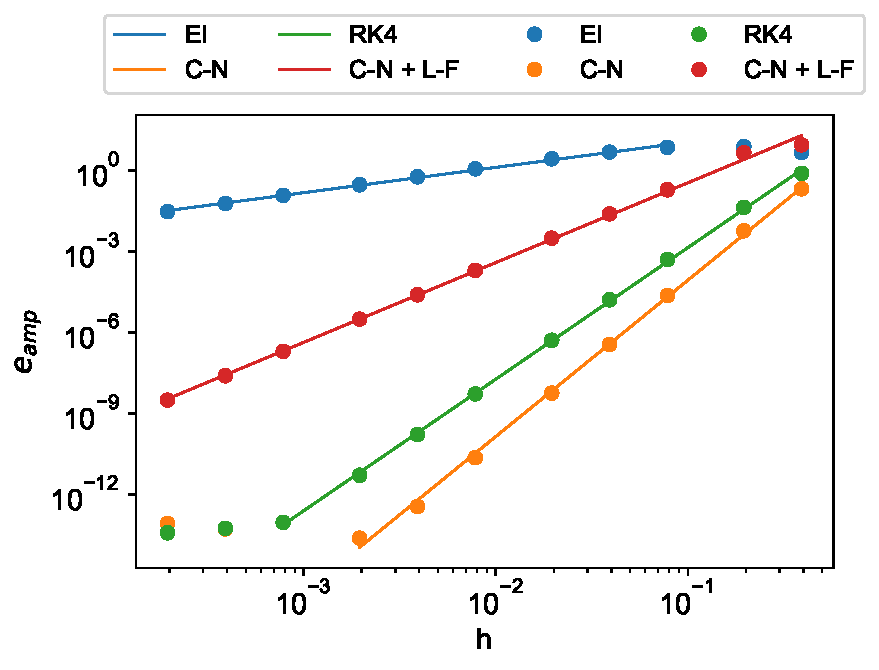
\includegraphics[clip=true,width=\columnwidth]{error_amplitud_simple_pi2.pdf}
%   \caption{Error de amplitud $e^S_{amp}$ para los cuatro esquemas numéricos en función del tamaño de la discretización $h$ bajo las condiciones iniciales $\theta_0 = \pi/2$. \textcolor{red}{Los puntos...}}
%    \label{fig:error_amplitud_simple_pi2}
% \end{figure}

% % AMPLITUD:
% % Orden de convergencia Euler implícito:  0.9372575985568138 +/- 0.01902503308713794, o sea, $0.94 \pm 0.02$
% % Orden de convergencia Crack-Nicholson:  5.790183279314054 +/- 0.09070012637078931, o sea, $5.79 \pm 0.09$
% % Orden de convergencia RK4:  4.872347720305063 +/- 0.03460069824650806, o sea, $4.87 \pm 0.04$
% % Orden de convergencia C-N + Leap-Frog:  2.9552896088114005 +/- 0.04216313986505771, o sea, $2.96 \pm 0.05%



% \begin{figure}[h]
%   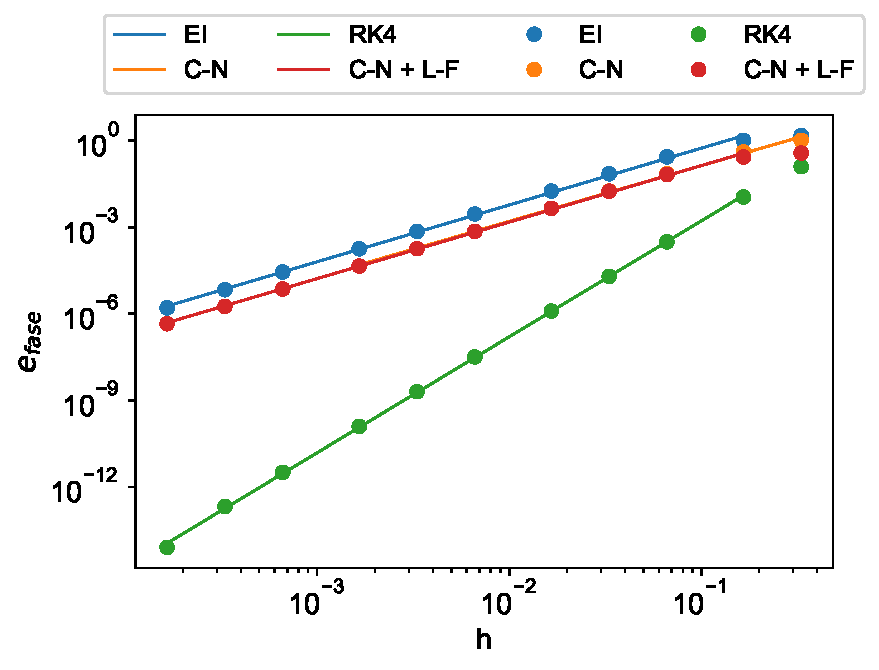
\includegraphics[clip=true,width=\columnwidth]{error_fase_simple_angulo_bajo.pdf}
%   \caption{\textcolor{blue}{(b) Error de amplitud para los 4 métodos para tita inicial de 10e-4}}
%    \label{fig:error_fase_simple_angulo_bajo}
% \end{figure}
% % FASE:
% % Orden de convergencia Euler implícito:  1.969515531340741 +/- 0.02352945286109731, o sea, $1.97 \pm 0.03$
% % Orden de convergencia Crack-Nicholson:  1.9315725179531302 +/- 0.031743969584564165, o sea, $1.93 \pm 0.04$
% % Orden de convergencia RK4:  4.020308658595079 +/- 0.020460933506094077, o sea, $4.02 \pm 0.02$
% % Orden de convergencia C-N + Leap-Frog:  1.9591911569629437 +/- 0.019303222788158225, o sea, $1.96 \pm 0.02$


% \begin{figure}[h]
%   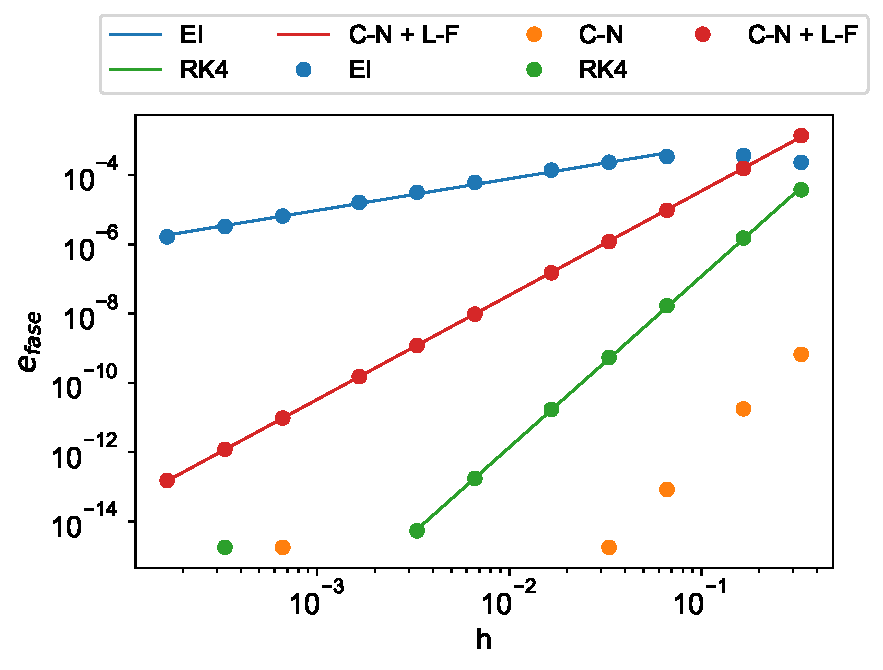
\includegraphics[clip=true,width=\columnwidth]{error_amplitud_simple_angulo_bajo.pdf}
%   \caption{\textcolor{blue}{(a) Error de fase para los 4 métodos para tita inicial de 10e-4}}
%    \label{fig:error_amplitud_simple_angulo_bajo}
% \end{figure}
% % AMPLITUD:
% % Orden de convergencia Euler implícito:  0.9125871407963045 +/- 0.023038374694042806, o sea, $0.91 \pm 0.03$
% % Orden de convergencia RK4:  4.940148423340664 +/- 0.023908301779203472, o sea, $4.94 \pm 0.03$
% % Orden de convergencia C-N + Leap-Frog:  3.0099767594644535 +/- 0.004694372715781479, o sea, $3.010 +/- 0.005$
% % CN tiene error cero creo

\onecolumngrid


\begin{figure}
  \centering
  \begin{subfigure}[b]{0.45\textwidth}
      \centering
      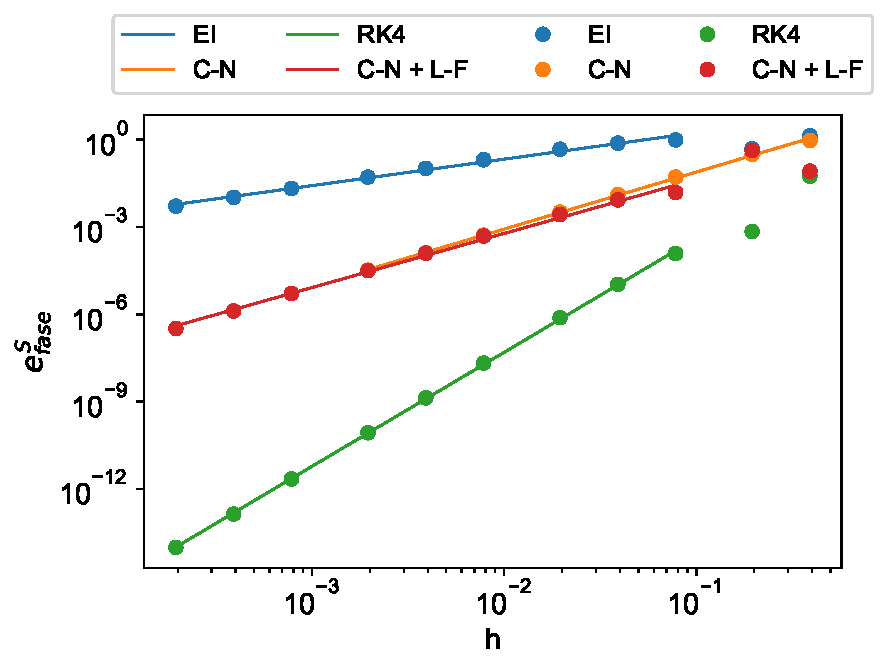
\includegraphics[width=\textwidth]{error_fase_simple_pi2.pdf}
      \caption{\label{fig:error_fase_simple_pi2}}
  \end{subfigure}
  \hfill
  \begin{subfigure}[b]{0.45\textwidth}
      \centering
      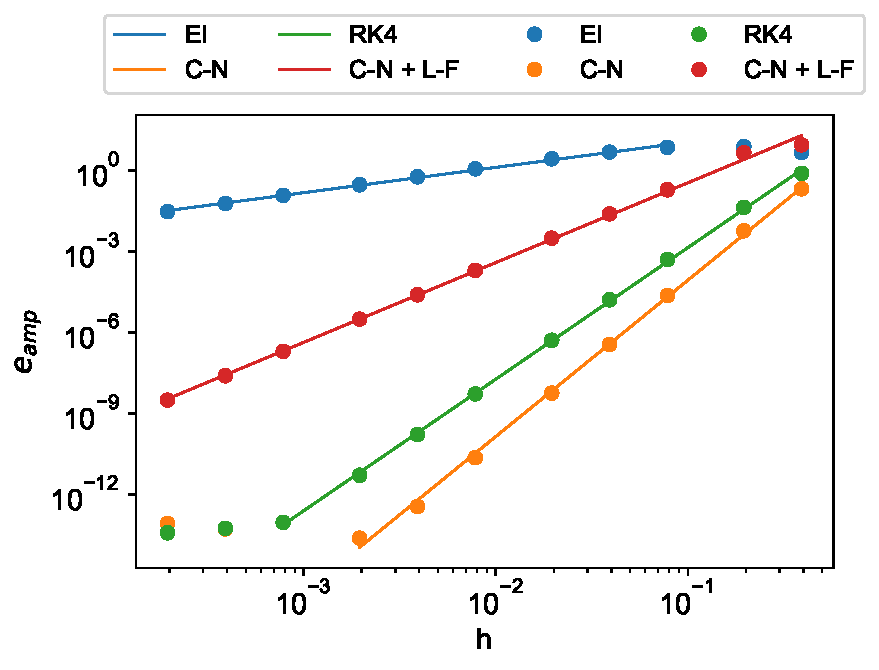
\includegraphics[width=\textwidth]{error_amplitud_simple_pi2.pdf}
      \caption{\label{fig:error_amplitud_simple_pi2}}
  \end{subfigure}
  \hfill
  \begin{subfigure}[b]{0.45\textwidth}
      \centering
      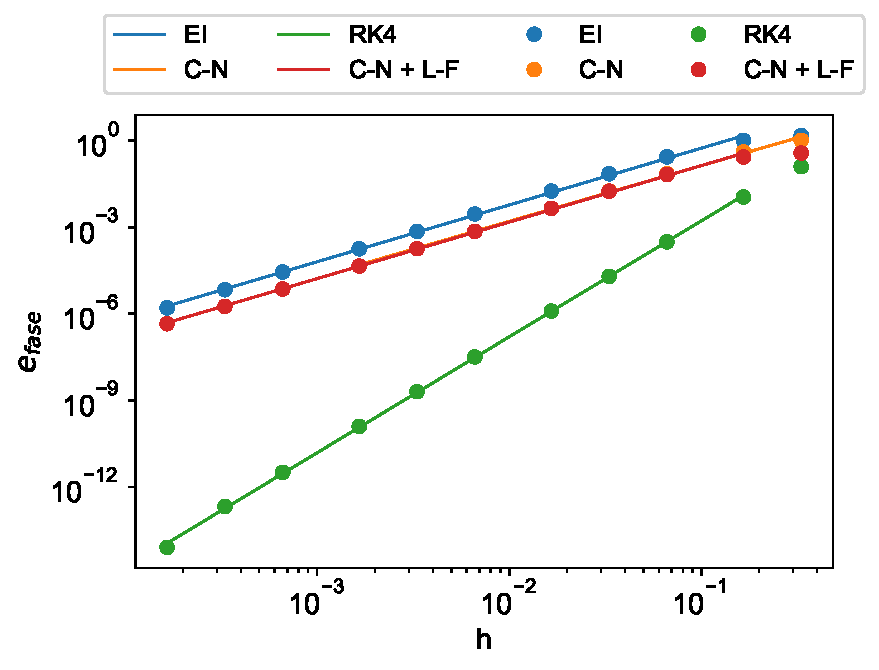
\includegraphics[width=\textwidth]{error_fase_simple_angulo_bajo.pdf}
      \caption{\label{fig:error_fase_simple_angulo_bajo}}
  \end{subfigure}
  \hfill
  \begin{subfigure}[b]{0.45\textwidth}
      \centering
      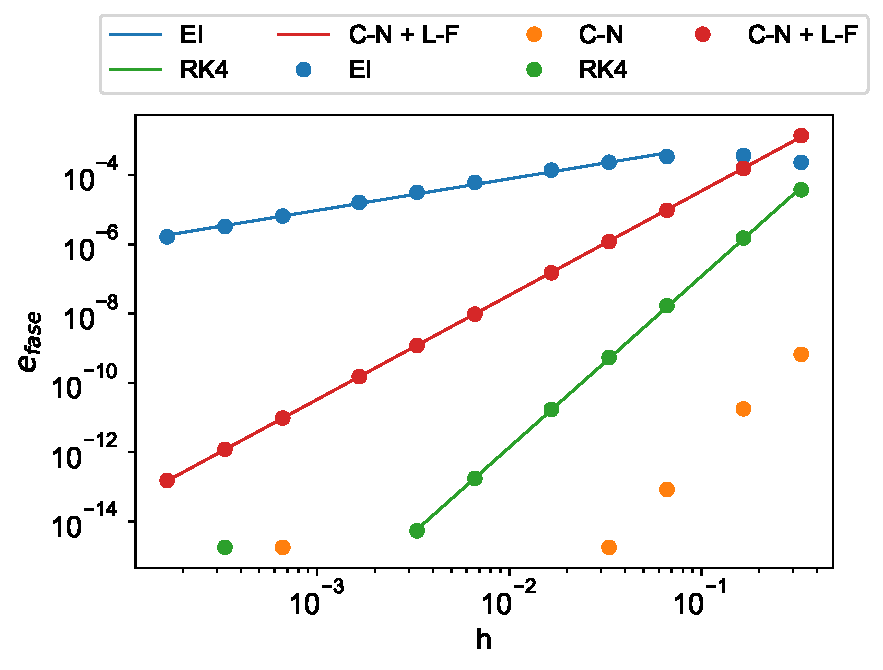
\includegraphics[width=\textwidth]{error_amplitud_simple_angulo_bajo.pdf}
      \caption{\label{fig:error_amplitud_simple_angulo_bajo}}
  \end{subfigure}
     \caption{Error de fase $e^S_{fase}$ y error de amplitud $e^S_{amp}$ en función del tamaño de la discretización $h$ para los cuatro esquemas numéricos bajo las condiciones iniciales \ref{fig:error_fase_simple_pi2} y \ref{fig:error_amplitud_simple_pi2}, $\theta_0 = \pi/2$ y $\theta'_0 = 0$, \ref{fig:error_fase_simple_angulo_bajo} y \ref{fig:error_amplitud_simple_angulo_bajo}, $\theta_0 = 0.01$ y $\theta'_0 = 0$ . Los puntos corresponden a los valores calculados y las líneas a los ajustes lineales. 'EI': Euler implícito, 'C-N': Crank-Nicholson, 'RK4': Runge-Kutta 4 y 'C-N + L-F': dos pasos con Crank Nicholson y uno con Leap-Frog. En la figura \ref{sub@fig:error_fase_simple_angulo_bajo} los valores correspondientes a CN y CN + LF se encuentran superpuestos.}
     \label{fig:simple_error_vs_h}
\end{figure}



\twocolumngrid



\onecolumngrid


% Please add the following required packages to your document preamble:
% \usepackage{multirow}
\begin{table}[]
  \begin{tabular}{|c|llllll|}
  \hline
  \multirow{3}{*}{Método} &
    \multicolumn{6}{c|}{Orden de convergencia de} \\ \cline{2-7} 
   &
    \multicolumn{3}{c|}{$e^S_{fase}$} &
    \multicolumn{3}{c|}{$e^S_{amp}$} \\ \cline{2-7} 
   &
    \multicolumn{1}{c|}{teórico} &
    \multicolumn{1}{c|}{con $\theta_0 = \pi/2$} &
    \multicolumn{1}{c|}{con $\theta_0 = 0.01$} &
    \multicolumn{1}{c|}{teórico} &
    \multicolumn{1}{c|}{con $\theta_0 = \pi/2$} &
    \multicolumn{1}{c|}{con $\theta_0 = 0.01$} \\ \hline
  EI &
    \multicolumn{1}{l|}{2} &
    \multicolumn{1}{l|}{$0.91 \pm 0.03$} &
    \multicolumn{1}{l|}{$1.97 \pm 0.03$} &
    \multicolumn{1}{l|}{1} &
    \multicolumn{1}{l|}{$0.94 \pm 0.02$} &
    $0.91 \pm 0.03$ \\ \hline
  CN &
    \multicolumn{1}{l|}{2} &
    \multicolumn{1}{l|}{$1.96 \pm 0.02$} &
    \multicolumn{1}{l|}{$1.93 \pm 0.04$} &
    \multicolumn{1}{l|}{error nulo} &
    \multicolumn{1}{l|}{$5.79 \pm 0.09$} &
    error nulo \\ \hline
  RK4 &
    \multicolumn{1}{l|}{4} &
    \multicolumn{1}{l|}{$3.92 \pm 0.02$} &
    \multicolumn{1}{l|}{$4.02 \pm 0.02$} &
    \multicolumn{1}{l|}{5} &
    \multicolumn{1}{l|}{$4.87 \pm 0.04$} &
    $4.94 \pm 0.03$ \\ \hline
  CN + LF &
    \multicolumn{1}{l|}{3} &
    \multicolumn{1}{l|}{$1.86 \pm 0.05$} &
    \multicolumn{1}{l|}{$1.96 \pm 0.02$} &
    \multicolumn{1}{l|}{error nulo} &
    \multicolumn{1}{l|}{$2.96 \pm 0.05$} &
    $3.010 \pm 0.005$ \\ \hline
  \end{tabular}
  \caption{\label{tabla:simple_errores} Orden de convergencial del error de fase $e^S_{fase}$ y del error de amplitud $e^S_{amp}$ para los cuatro esquemas numéricos bajo las condiciones iniciales $\theta'_0 = 0$ y distintos valores de $\theta_0$. 'EI': Euler implícito, 'C-N': Crank-Nicholson, 'RK4': Runge-Kutta 4 y 'C-N + L-F': dos pasos con Crank Nicholson y uno con Leap-Frog. Los valores teóricos provienen fueron extraídos de \cite{Notas_materia}.}
  \end{table}

\twocolumngrid


\hfill

En base al comportamiento lineal se realizó un ajuste lineal y se obtuvieron los órdenes de convergencia. Los resultados se resumen en la tabla \ref{tabla:simple_errores}. En cuanto a $e^S_{fase}$, los órdenes teóricos y numéricos son indistinguibles considerando dos desviaciones estándard para EI, CN y RK4. Esto es acorde a la hipótesis sobre $\theta_0$ planteada. Sin embargo, no se obtiene el valor esperado para el método CN + LF. Esto se podría deber a que el error de fase en el problema no lineal no resulta de orden 3, sino que se mantiene en orden 2. Para ser válido el orden 3 se deberían compensar los errores de fase de cada método mutuamente, para lo cual también es necesario que el error de fase no dependa del paso de integración. Esto podría no ser cierto para el problema no lineal y por lo tanto sería razonable mantener el orden 2.

En cuanto a $e^S_{amp}$, los órdenes teóricos y numéricos son indistinguibles considerando dos desviaciones estándard para CN y RK4. Sin embargo, este no es el caso de EI y CN + LF. No es claro a qué se deben ambos comportamientos. Debería estudiarse este problema con mayor detalle. Una opción posible sería considerar $\theta_0$ menor al utilizado. Esto no es factible de realizar en Octave debido a un problema de representación decimal en el lenguaje de programación.





\subsection{Péndulo doble}

Se resolvió el sistema \ref{eq:pendulo_doble_vec} empleando el método RK4 y se estudió la sensibilidad del sistema frente a perturbaciones, la posibilidad de identificar patrones en la trayectoria de las partículas que conforman el péndulo y la conservación de la energía


En primer lugar, se evaluó la sensibilidad del sistema frente a perturbaciones sobre las condiciones iniciales. Para esto se calculó la dinámica del péndulo doble para tres condiciones iniciales ligeramente distintas: $\theta_{1 0} = \pi/2$, $\theta_{2 0} = a$ y $\theta'_{1 0} = \theta'_{2 0} = 0$ con $a^A = \pi/2$, $a^B = 1.00001 \pi/2$ y $a^C = 0.99999 \pi/2$. Para la evolución numérica se empleó $h = \pi/100 \approx 0.0314$. En la figura \ref{fig:doble_3CI} se grafica la evolución de $\theta_1(t)$. Se observa que la evolución es similar para las tres condiciones iniciales hasta $t \approx 5 \pi$ cuando comienzan a diferir considerablemente. Esta diferencia se podría justificar en una sensibilidad frente a las condiciones iniciales o bien a errores del método numérico utilizado. En base a esto se calcularon las diferencias angulares entre las soluciones para $\theta_1$ y $\theta_2$, en función de $h$ a $t = 5 \pi$. Los resultados se grafican en la figura \ref{fig:doble_3CI_difs}. Se observa que la diferencia entre las soluciones se mantiene constante a partir de un valor de $h$ suficientemente pequeño. Por lo tanto, las diferencias no se deben al método numérico y el sistema es sensible a las perturbaciones

\begin{figure}[h]
  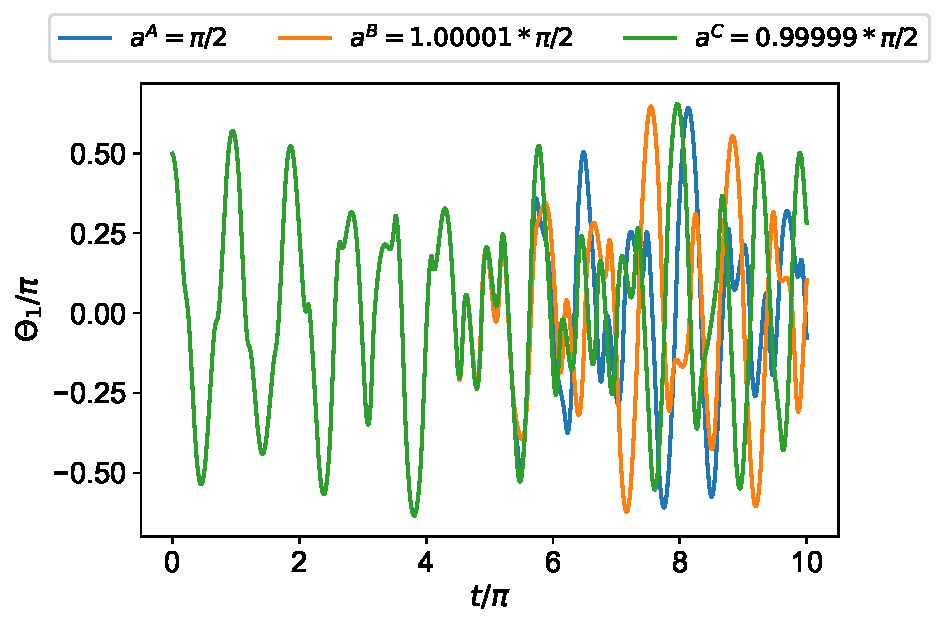
\includegraphics[clip=true,width=\columnwidth]{doble_3CI.pdf}
  \caption{Evolución de $\theta_1(t)$ para los cuatro esquemas numéricos para las condiciones iniciales $\theta_{1 0} = \pi/2$, $\theta_{2 0} = a$ y $\theta'_{1 0} = \theta'_{2 0} = 0$ con $h = \pi/100$. Ambos ejes se encuentran normalizados por $\pi$. La evolución se realizó mediante el método numérico Runge-Kutta 4.}
   \label{fig:doble_3CI}
\end{figure}


\begin{figure}[h]
  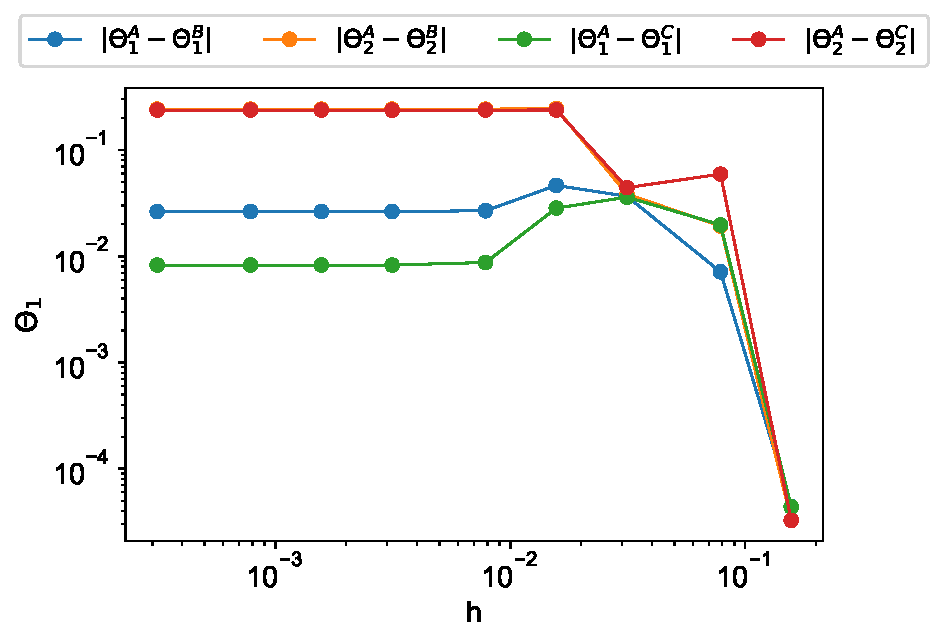
\includegraphics[clip=true,width=\columnwidth]{doble_3CI_difs.pdf}
  \caption{Diferencias angulares entre soluciones numéricas con distintas condiciones iniciales a tiempo $t = 5 \pi$, en función de h. Las condiciones iniciales corresponden a $\theta_{1 0} = \pi/2$, $\theta_{2 0} = a$ y $\theta'_{1 0} = \theta'_{2 0} = 0$ con $a^A = \pi/2$, $a^B = 1.00001 \pi/2$ y $a^C = 0.99999 \pi/2$. La evolución se realizó mediante el método numérico Runge-Kutta 4.}
   \label{fig:doble_3CI_difs}
\end{figure}

\begin{figure}[h]
  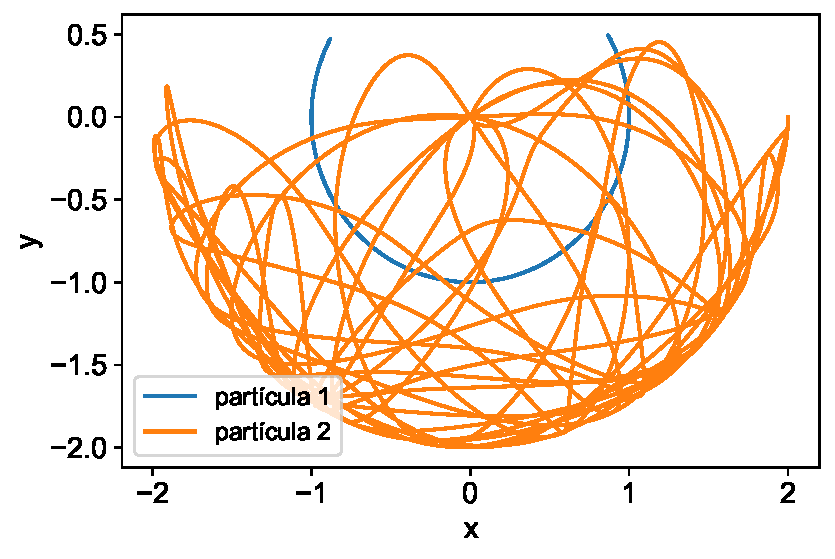
\includegraphics[clip=true,width=\columnwidth]{doble_1CI_trayectorias.pdf}
  \caption{Trayectorias de las dos partículas de un péndulo doble para las condiciones iniciales  $\theta_{1 0} = \theta_{2 0} = \pi/2$ y $\theta'_{1 0} = \theta'_{2 0} = 0$, bajo la discretización $h = \pi/1000$ e intervalo de tiempo $t \in [0, 10 \pi]$. La evolución se realizó mediante el método numérico Runge-Kutta 4.}
   \label{fig:doble_1CI_trayectorias}
\end{figure}

En segundo lugar, se calculó la trayectoria de las partículas que conforman el péndulo doble para las condiciones iniciales $\theta_{1 0} = \theta_{2 0} = \pi/2$ y $\theta'_{1 0} = \theta'_{2 0} = 0$, discretización $h = \pi/1000$ e intervalo de tiempo $t \in [0, 10 \pi]$. Tales trayectorias se grafican en la figura \ref{fig:doble_1CI_trayectorias}. La trayectoria de la partícula 1 está restringida a una circunferencia de radio 1 alrededor del origen. Mientras que la de la partícula 2 tiene mayor libertad de movimiento, no observándose patrones claros en el comportamiento del péndulo.


\begin{figure}
  \centering
  \begin{subfigure}[b]{0.45\textwidth}
      \centering
      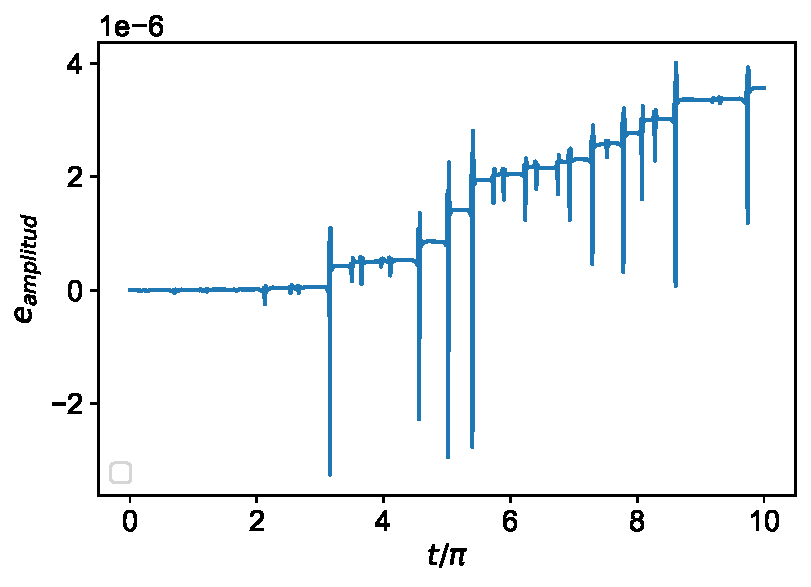
\includegraphics[width=\textwidth]{doble_error_amplitud.pdf}
      \caption{\label{fig:doble_error_amplitud}}
  \end{subfigure}
  \hfill
  \begin{subfigure}[b]{0.45\textwidth}
      \centering
      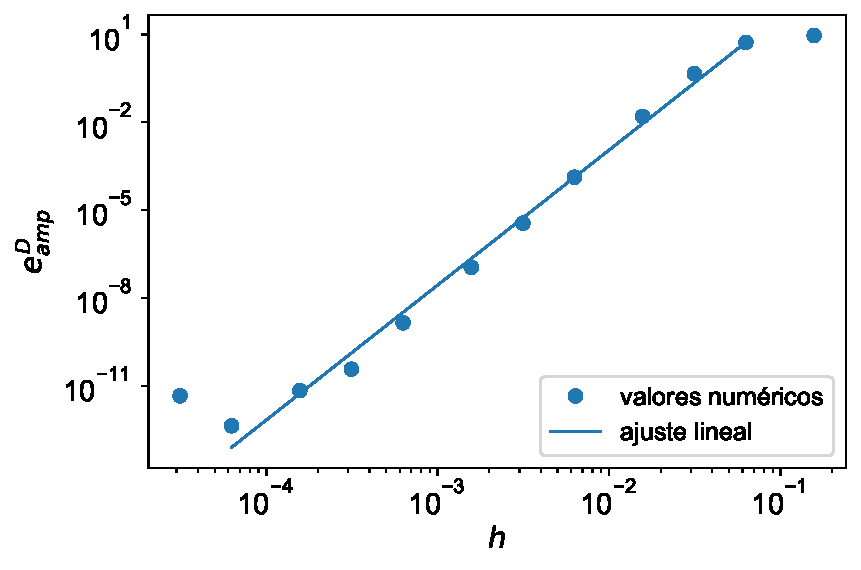
\includegraphics[width=\textwidth]{doble_orden_error_amplitud.pdf}
      \caption{\label{fig:doble_orden_error_amplitud}}
  \end{subfigure}
     \caption{\ref{fig:doble_error_amplitud} error de amplitud  $e_{amp}^D$ en función del tiempo $t$. \ref{fig:doble_orden_error_amplitud} error de amplitud  $e_{amp}^D$ en función del tamaño de la discretización $h$. Ambos cálculos se realizaron para las condiciones iniciales $\theta_{1 0} = \theta_{2 0} = \pi/2$ y $\theta'_{1 0} = \theta'_{2 0} = 0$, discretización $h = \pi/1000$ e intervalo de tiempo $t \in [0, 10 \pi]$. La evolución se realizó mediante el método numérico Runge-Kutta 4.}
     \label{fig:doble_e_amp}
\end{figure}


En tercer lugar, se calculó la energía del sistema para las mismas condiciones iniciales y discretización que en el caso anterior. Se calculó el error de amplitud $e_{amp}^D$ a partir de la expresión \ref{eq:doble_e_amp} y se graficó en función del tiempo en la figura \ref{fig:doble_error_amplitud}. Se observa que la amplitud no se converva, aunque el error es relativamente pequeño. En base a esto, se buscó determinar el error de convergencia, calculando $e_{amp}^D$ en función de $h$. Los resultados se grafican en la figura \ref{fig:doble_orden_error_amplitud}. Se distinguen tres regiones. Inicialmente, para $h$ grande,
el error presenta un comportamiento aleatorio. A medida que $h$ disminuye, el error varía como una potencia de $h$, es decir, de forma lineal en escala logarítmica. Por
último, para valores de $h$ menores, el error aumenta debido a los errores de precisión de la computadora. En base al comportamiento en la región central se realiza un ajuste lineal cuya pendiente $m = 4.6 \pm 0.2$ corresponde al orden de convergencia. Este valor no es consistente con el error teórico de orden $5$, aunque la diferencia se podría justificar en el comportamiento no lineal del sistema.




% \begin{figure}[h]
%   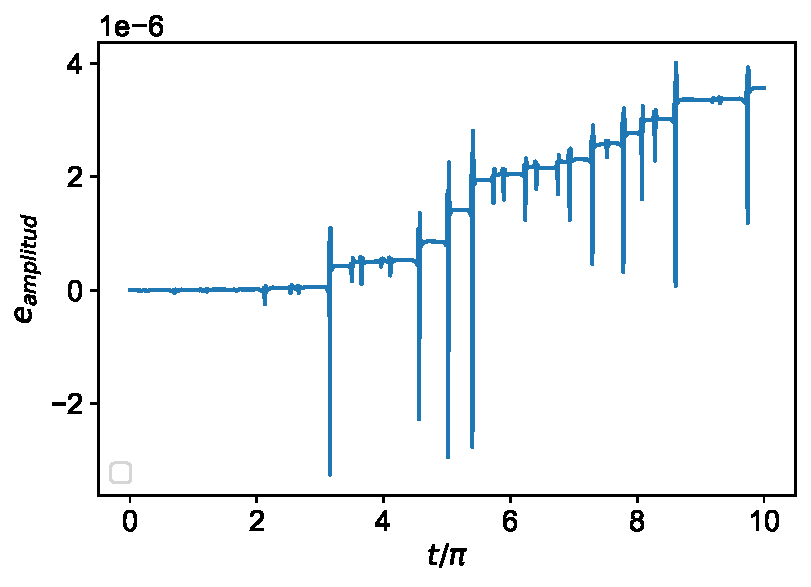
\includegraphics[clip=true,width=\columnwidth]{doble_error_amplitud.pdf}
%   \caption{Error de amplitud  $e_{amp}^D$ en función del tiempo $t$. Error de amplitud  $e_{amp}^D$ en función del tamaño de la discretización $h$. Ambos cálculos se realizaron para las condiciones iniciales $\theta_{1 0} = \theta_{2 0} = \pi/2$ y $\theta'_{1 0} = \theta'_{2 0} = 0$, discretización $h = \pi/1000$ e intervalo de tiempo $t \in [0, 10 \pi]$. La evolución se realizó mediante el método numérico Runge-Kutta 4.}
%    \label{fig:doble_error_amplitud.pdf}
% \end{figure}

% \begin{figure}[h]
%   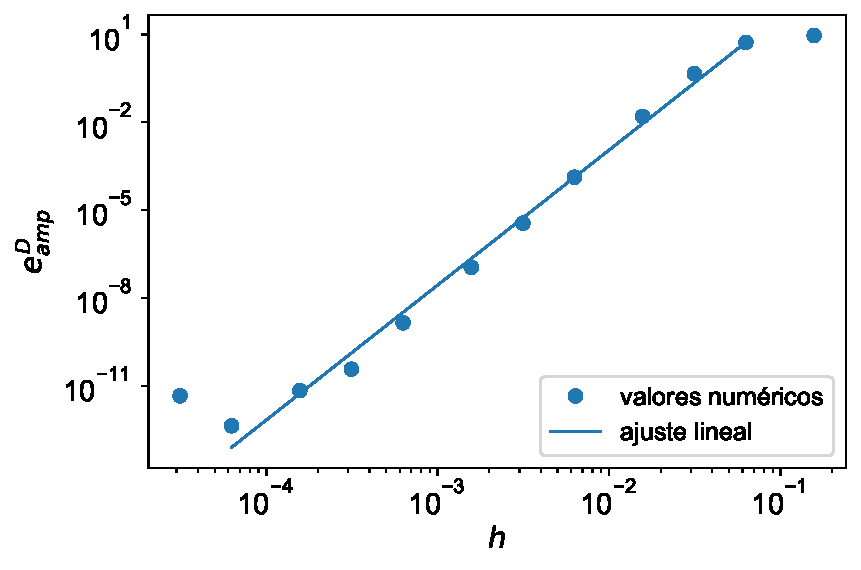
\includegraphics[clip=true,width=\columnwidth]{doble_orden_error_amplitud.pdf}
%   \caption{\textcolor{blue}{Orden del error de amplitud}}
%    \label{fig:doble_orden_error_amplitud}
% \end{figure}


\section{Conclusión}

Se estudiaron distintos métodos numéricos para resolver problemas de valores iniciales no lineales. En primer lugar, se aplicaron los métodos de Euler implícito, Crank-Nicholson, Runge-Kutta 4 y una combinación de Crank-Nicholson con Leap-Frog al problema del péndulo simple. El último método se propuso con el objetivo de obtener un error de fase de mayor orden que los métodos por separado. Se analizaron los errores de fase y amplitud globales de cada método, se calcularon los órdenes de convergencia y se compararon con los valores teóricos, calculados en base a un problema lineal. En cuanto al error de fase, se encontraron valores similares a los teóricos, salvo para la combinación de Crank-Nicholson y Leap-Frog. Se encontró que el error no aumenta de orden debido a que en problemas no lineales el error de fase depende del paso de tiempo y la compensación esperada no ocurre. En cuanto al de amplitud, se encontraron valores similares a los teóricos, salvo para el método de Crank-Nicholson y la combinación de este con Leap-Frog. En ambos casos se hubiera esperado encontrar error nulo y no fue así. La razón de este comportamiento podría deberse a la no linealidad del problema. En base a esto, debería recuperarse el comportamiento teórico para el péndulo simple con ángulo bajo. Esto ocurre para el método de Crank-Nisholson pero no para la combinación de métodos. Debería estudiarse este caso en particular con mayor detalle. 

En segundo lugar, se aplicó el método Runge-Kutta 4 para el problema del péndulo doble. Se obtuvo una gran sensibilidad del sistema frente a perturbaciones de las condiciones iniciales. Además, se observó la dificultad de reconocer patrones sobre las trayectorias de las partículas. Por último, se encontró que la energía proporcional a la amplitud no se conserva. Se encontró un orden de convergencia para el error de amplitud distinto al valor teórico. Tal discrepancia se podría justificar con la misma razón que el péndulo simple: el sistema analizado es no lineal y los valores teóricos se calculan sobre problemas lineales.


\bibliography{Chehade_guia2.bib}

\end{document}





